\begin{figure}[!htbp]
  \centering
  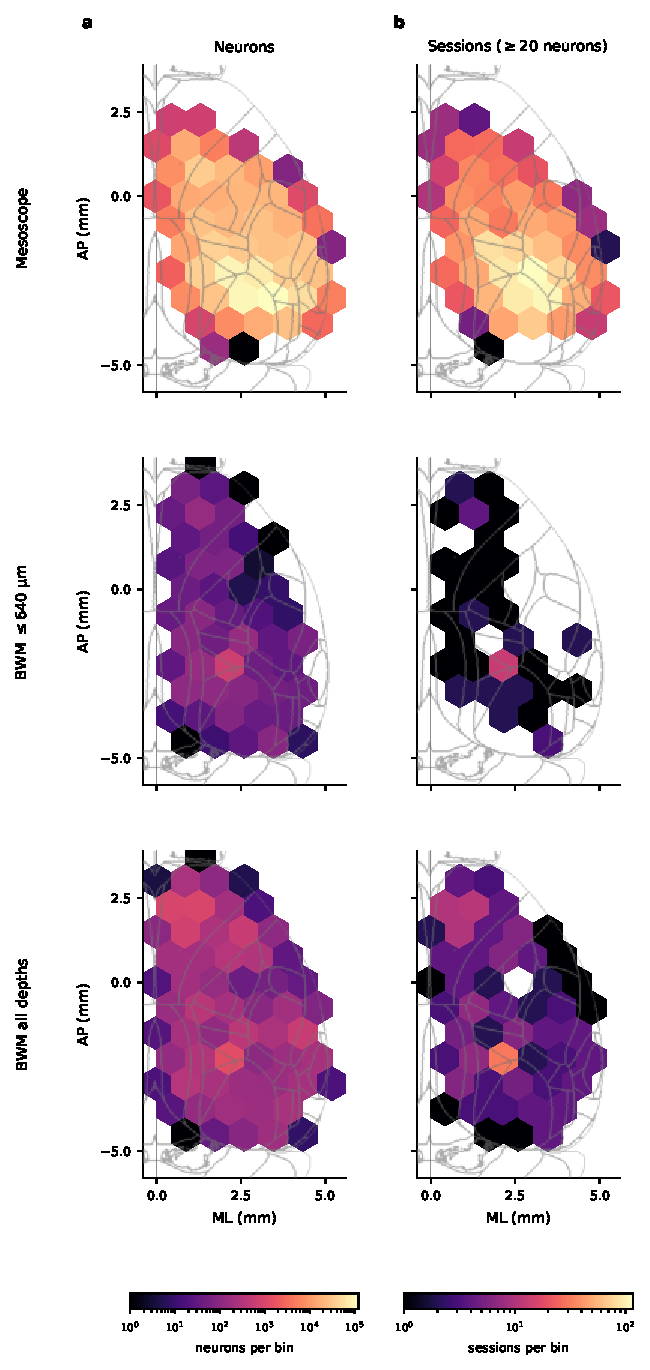
\includegraphics[width=4.32in,height=0.8\textheight,keepaspectratio]{figures/counts.pdf}
  \caption{Coverage: mesoscope two-photon imaging (top row; deconvolved activity of isocortex neurons) vs Brain Wide Map Neuropixels units within 640\,$\mu$m of the pial surface (middle row; twice the depth range the mesoscope images, 174--318\,$\mu$m) and at all depths (bottom row; reference). Each neuron is assigned to a hexagonal bin (1\,mm vertex to vertex) by its ML and AP Allen CCF position; hemispheres folded onto the right. Grey lines: Allen top-view region boundaries. Colour scales are shared across rows. \textbf{a} Number of isocortex neurons per bin: mesoscope 1,071,534 neurons, 151 sessions; BWM $\leq$640\,$\mu$m 2,929 neurons, 204 sessions; BWM all depths 13,002 neurons, 288 sessions. \textbf{b} Number of sessions contributing at least 20 neurons to each bin.}
  \label{fig:counts}
\end{figure}
